% Options for packages loaded elsewhere
\PassOptionsToPackage{unicode}{hyperref}
\PassOptionsToPackage{hyphens}{url}
\PassOptionsToPackage{dvipsnames,svgnames*,x11names*}{xcolor}
%
\documentclass[
  12pt,
]{article}
\usepackage{lmodern}
\usepackage{setspace}
\usepackage{amssymb,amsmath}
\usepackage{ifxetex,ifluatex}
\ifnum 0\ifxetex 1\fi\ifluatex 1\fi=0 % if pdftex
  \usepackage[T1]{fontenc}
  \usepackage[utf8]{inputenc}
  \usepackage{textcomp} % provide euro and other symbols
\else % if luatex or xetex
  \usepackage{unicode-math}
  \defaultfontfeatures{Scale=MatchLowercase}
  \defaultfontfeatures[\rmfamily]{Ligatures=TeX,Scale=1}
  \setmainfont[]{Times New Roman}
  \setsansfont[]{Times New Roman}
\fi
% Use upquote if available, for straight quotes in verbatim environments
\IfFileExists{upquote.sty}{\usepackage{upquote}}{}
\IfFileExists{microtype.sty}{% use microtype if available
  \usepackage[]{microtype}
  \UseMicrotypeSet[protrusion]{basicmath} % disable protrusion for tt fonts
}{}
\makeatletter
\@ifundefined{KOMAClassName}{% if non-KOMA class
  \IfFileExists{parskip.sty}{%
    \usepackage{parskip}
  }{% else
    \setlength{\parindent}{0pt}
    \setlength{\parskip}{6pt plus 2pt minus 1pt}}
}{% if KOMA class
  \KOMAoptions{parskip=half}}
\makeatother
\usepackage{xcolor}
\IfFileExists{xurl.sty}{\usepackage{xurl}}{} % add URL line breaks if available
\IfFileExists{bookmark.sty}{\usepackage{bookmark}}{\usepackage{hyperref}}
\hypersetup{
  colorlinks=true,
  linkcolor=Maroon,
  filecolor=Maroon,
  citecolor=Blue,
  urlcolor=Blue,
  pdfcreator={LaTeX via pandoc}}
\urlstyle{same} % disable monospaced font for URLs
\usepackage[margin=1in]{geometry}
\usepackage{longtable,booktabs}
% Correct order of tables after \paragraph or \subparagraph
\usepackage{etoolbox}
\makeatletter
\patchcmd\longtable{\par}{\if@noskipsec\mbox{}\fi\par}{}{}
\makeatother
% Allow footnotes in longtable head/foot
\IfFileExists{footnotehyper.sty}{\usepackage{footnotehyper}}{\usepackage{footnote}}
\makesavenoteenv{longtable}
\usepackage{graphicx,grffile}
\makeatletter
\def\maxwidth{\ifdim\Gin@nat@width>\linewidth\linewidth\else\Gin@nat@width\fi}
\def\maxheight{\ifdim\Gin@nat@height>\textheight\textheight\else\Gin@nat@height\fi}
\makeatother
% Scale images if necessary, so that they will not overflow the page
% margins by default, and it is still possible to overwrite the defaults
% using explicit options in \includegraphics[width, height, ...]{}
\setkeys{Gin}{width=\maxwidth,height=\maxheight,keepaspectratio}
% Set default figure placement to htbp
\makeatletter
\def\fps@figure{htbp}
\makeatother
\setlength{\emergencystretch}{3em} % prevent overfull lines
\providecommand{\tightlist}{%
  \setlength{\itemsep}{0pt}\setlength{\parskip}{0pt}}
\setcounter{secnumdepth}{5}
\usepackage{mathtools}

\title{\vspace{1cm}Does Spending time with your child decreases your income?\vspace{0.5cm}\\}
\author{Sophie Hensgen\\
University of Mannheim\\
Matricle number: 1560750}
\date{2020-07-13\\}

\begin{document}
\maketitle
\begin{abstract}
\noindent\setstretch{1}Here Abstract\ldots{}\vspace{.8cm}
\end{abstract}

\setstretch{1.2}
\hypertarget{introduction}{%
\section{Introduction}\label{introduction}}

(Evertsson \protect\hyperlink{ref-evertsson_parental_2016}{2016})

\hypertarget{literature-review}{%
\section{Literature Review}\label{literature-review}}

\hypertarget{history-of-parental-leave}{%
\subsubsection*{\texorpdfstring{\emph{History of Parental Leave}}{History of Parental Leave}}\label{history-of-parental-leave}}
\addcontentsline{toc}{subsubsection}{\emph{History of Parental Leave}}

In order to fully understand the impact maternity, paternity and parental leave might have on an individual, it is necessary to look into the reform itself and how it changed over the years to become more inclusive. Maternity leave itself did not changed as much, women were guaranteed 14 weeks of leave (6 weeks pre birth and 8 post birth) with full payment of their salary (Gabriele Mari and Cutuli \protect\hyperlink{ref-gabriele_mari_parental_2019}{2019}). In the 1980s in Germany, mothers were offered 6 months of paid and job guaranteed leave. This reform has been amended several times. Especially in the 1990s they started to change the status quo quite a bit. Not only changed the period of time during which a safe return to work was guaranteed to 36 months in 1992. But also they adjusted the financial support in the same year so that it could be paid for 18 months. This financial support consisted of a mixture of flat-rate and means-tested payments (Gabriele Mari and Cutuli \protect\hyperlink{ref-gabriele_mari_parental_2019}{2019}). Another rather big change was the possibility that both parents could simultaneously go into parental leave {[}geisler\_against\_2011; Bundesministerium{]}.
The next big reform change took place in 2007. The paid leave was at least 12 months and 14 if both parents at least took two weeks parental leave. These additional 2 months should act like an incentive for fathers to take part in parental leave (Gabriele Mari and Cutuli \protect\hyperlink{ref-gabriele_mari_parental_2019}{2019}; Lapuerta, Baizán, and González \protect\hyperlink{ref-lapuerta_individual_2011}{2011}; Marshall \protect\hyperlink{ref-marshall_fathers_2008}{2008}). Also the financial support system changed. If someone was employed to the time of the birth they would get paid 67 \% of their pre-birth net salary. But if you were not employed you get 300 Euro per month as financial support (Hofferth and Curtin \protect\hyperlink{ref-hofferth_parental_2006}{2006}).
These reform changes have a strong influence on the likelihood of fathers taking parental leave. Before 2007, only 3\% of fathers took parental leave. After 2007, the figure had already risen to 15\%, increasing over the years to 34\% (2014) (Tamm \protect\hyperlink{ref-tamm_fathers_2018}{2018}).
Mari \& Cutuliy examined the impact the 2007 reform had on the income of parents and they found out that indeed, more fathers engaged in parental leave and also that it was easier to return to the job market for women.
For the rest of the paper, I am going to focus on the reforms of 1992 \& 1993, cohabiting was not allowed, as well as no additional 2 months of parental leave for the father.

\hypertarget{theory-hypotheses}{%
\section{Theory \& Hypotheses}\label{theory-hypotheses}}

\hypertarget{impact-of-parental-leave}{%
\subsubsection*{\texorpdfstring{\emph{Impact of Parental Leave}}{Impact of Parental Leave}}\label{impact-of-parental-leave}}
\addcontentsline{toc}{subsubsection}{\emph{Impact of Parental Leave}}

According to multiple scholars, there seems to be a significant influence of parental leave on income in varing degrees.
However it is important to note that there are two aspects that are decisive for this research field. First, there are aspects which influence the decision to go into parental leave, which can lead to the overrepresentation of women staying home for their newborn. And second, parental leave in general will have an influence, which can be harder on one parent, but other parts should not be affected by the gender. In the following section I will first concentrate on what is going into the deciding process on who should go into parenta leave of the two of them and for how long. And then, I will explore the different reasons for the disadvantages which come with parental leave.

Taking time to nurture your new born child is an important aspect in the relationship between parents and their child. For a lot of people it is without question that they will partake in parental leave, even for a longer period of time. However, when it comes to any kind of parental leave, there are several things to consider before deciding who is going to take it and also for how long. In general people are quite rational about it, they weigh their costs according to the economic theory (Lapuerta et al. \protect\hyperlink{ref-lapuerta_individual_2011}{2011}), so their outcome will be the best way possible in regards to finances, reentry in work force etc.. For example, parents look into the labor market and their own company to find out, if the situation is stable and which is best to leave for a period of time (Sundstrom \protect\hyperlink{ref-sundstrom_gender_2002}{2002}). However, some decisions which are made during this time even if chosen rationally can lead to disadvantages, for one party. In particular women, research shows that first time parents tend to engage in a more traditional constellation {[}dribe\_does\_2009{]}.

However these decisions are made on basis of multiple criteria, not only because of stereotypes. 6 of them seem to be especially prominent during the decision process.
To begin with the perhaps least crucial criteria is the lifestyle preferences of each individual. For some, work is more important, for some it is the family, for others it is a matter of adapting to the situation. Depending on which side one is on, this can influence the willingness to take parental leave and also the extent to which it is taken {[}Hofferth and Curtin (\protect\hyperlink{ref-hofferth_parental_2006}{2006}); Hakim{]}.\\
Another aspect I mentioned shortly before is the situation of the labor market. Some parents are worried, that if they take parental leave, they could have disadvantages compared to other workers in this field. Additionally, some markets are more stable than other, so if someone has a secure job, they might want to stay working to show their commitment (Sundstrom \protect\hyperlink{ref-sundstrom_gender_2002}{2002}).
However, this might not be the most influential part, as these concerns are closely linked with the reform which is in action. Parental leave programs are different in each country, some are more flexible (Finland, Germany), some are not (Spain, Italy, Greece) (Gabriele Mari and Cutuli \protect\hyperlink{ref-gabriele_mari_parental_2019}{2019}; Pronzato \protect\hyperlink{ref-pronzato_return_2009}{2009}; Tamm \protect\hyperlink{ref-tamm_fathers_2018}{2018}). And if they are more flexible, the probability that fathers will take parental leave will increase. (Gabriele Mari and Cutuli \protect\hyperlink{ref-gabriele_mari_parental_2019}{2019})
Still, the rate of father who partake in parental leave is still small, as the society still expect women to at least stay home at the beginning (Cite; Katherine Marshall \protect\hyperlink{ref-katherine_marshall_fathers_2008}{2008}). This does not necessarily have to have anything to do with sexism and stereotypes, although they do have an impact (Evertsson \protect\hyperlink{ref-evertsson_parental_2016}{2016}) (read again), but there are practical reasons as well. The woman carries the child, gives birth and would probably also breastfeed it in the first couple of months, if she decide to do so. Therefore it makes sense that the mother stays at home with the child at the beginning. However, this does not explain, why women stay even longer even though both parents could technically care for the child.
We can see a trend away from the traditional route, especially for higher educated parents. Even though high educated people have higher opportunity cost as they could potentially improve their career easier and thus partake less in parental leave and if so for a shorter amount of time (Helen Dearing \protect\hyperlink{ref-helen_dearing_does_2015}{2015}; Lapuerta et al. \protect\hyperlink{ref-lapuerta_individual_2011}{2011}; Rostgaard, Christoffersen, and Weise \protect\hyperlink{ref-rostgaard_parental_2020}{2020}). They are more willing to give up hetero-normative standards and adopting more egalitarian gender roles. Which means, that they do not have a problem to partake in parental leave (Geisler and Kreyenfeld \protect\hyperlink{ref-geisler_against_2011}{2011}).
With that said, there is one important aspect to note. Even though highly educated men are open to the idea of taking parental leave, it is important, that it is conform with the economic theory. Which means that they are more likely to go into parental leave, if their significant other has a higher education or higher income than themselves (Geisler and Kreyenfeld \protect\hyperlink{ref-geisler_against_2011}{2011}; Lapuerta et al. \protect\hyperlink{ref-lapuerta_individual_2011}{2011}; Tamm \protect\hyperlink{ref-tamm_fathers_2018}{2018}).
Income seems to be the most important criterion in relation to parental leave. It not only determines who takes it. but also how long the parental leave will last. High-income families can afford to take more time off for parental leave because they do not need a full additional income (Geisler and Kreyenfeld \protect\hyperlink{ref-geisler_against_2011}{2011}).

When the decision is made on who is going to stay home, other additional factors will potentially influence the income as well.\\
One of these disadvantages which come with staying home is the missed opportunities at work. Companys are fast changing mechanisms, new structures, workflows and task are added constantly. So missing out on these, even for a small period of time, could be harmful for one's career (Evertsson \protect\hyperlink{ref-evertsson_parental_2016}{2016}). These findings are in line with the human capital theory which states that an individual will increase its knowledge and skills through education and working in a specific field. The longer someone has been working and the more supplementary training and task he completed the higher his or hers human capital will be (Becker \protect\hyperlink{ref-becker_human_1993}{1993}; Evertsson \protect\hyperlink{ref-evertsson_parental_2016}{2016}). A high human capital is especially important to receive great job offerings, a high salary and promotions. Thus a break in work life can act like a bump on the career and put someone behind compared to those who did work constantly. Furthermore, the human capital is not only not increasing while staying home, in fact it is decreasing because of the lack of practice (Evertsson \protect\hyperlink{ref-evertsson_parental_2016}{2016}). This assumption is supported by the study by Hofferth and Curtin (Hofferth and Curtin \protect\hyperlink{ref-hofferth_parental_2006}{2006}). In their results, they found evidence that the salary already decreases 2 years after birth when the employer is changed. Although they have only focused on the impact on women, there are studies like Evertson's (Evertsson \protect\hyperlink{ref-evertsson_parental_2016}{2016}) which show that both women and men suffer a loss of pay after parental leave.
However, the well being of the child is most important for the parents, and they will only return to work, if it is more valuable for the family when him or her spends time working (especially regarding the salary) instead of carrying for the child {[}Hofferth and Curtin (\protect\hyperlink{ref-hofferth_parental_2006}{2006}); (Desai \& Waite, 1991; Joesch, 1994; Leibowitz, Klerman, \& Waite, 1992){]}.
How great the impact of parental leave has on the human capital and therefore on the income depends heavily on the reforms stated in each country. For example Pronzato (Pronzato \protect\hyperlink{ref-pronzato_return_2009}{2009}) examined multiple European countries and observed that in countries with more generous parental leave arrangements, like Finland the impact the leave had on the human capital was less severe as in other countries (Italy or Spain). So even though there is so much research in this field, every country reacts differently to parental leave depending on the reform in action. And as mentioned before even within countries there are changes in reforms, which change how people react to parental leave all together (ELEFANT change sentence, not happy with it).

So far we explored the impact parental leave can have on human capital, however there is another important aspect which is effected by parental leave, and that is signalling. According to signal theory, any action we take send out a signal that allows others to build up certain beliefs about us {[}Hedström{]}. In line with previous research, this means that parental leave can be a signal of less commitment to the company and its work, at least employers will interpret it like that (Sundstrom \protect\hyperlink{ref-sundstrom_gender_2002}{2002}). However, this seems to be more a problem for men than for women. This is because the expectation that women will take more care of their newborn child than their husbands is still widespread in society. 25\% of all couples do not even consider the possibility that the man could take parental leave (Rostgaard et al. \protect\hyperlink{ref-rostgaard_parental_2020}{2020}). It is so normalized, that the signal a women gives with taking maternity leave is not that severe and should not influence her income as much (Evertsson \protect\hyperlink{ref-evertsson_parental_2016}{2016}). However, if a man decides to take parental leave, it is still seen as an exception. Especially in the period before 2007 where additional incentives were included for men. So any time spend in parental leave will signal the employer less determination for the company and is also taken more seriously than if women took parental leave, which concludes in a greater impact on the men career and income (Evertsson \protect\hyperlink{ref-evertsson_parental_2016}{2016}, albrecht\_career\_1999). In a Swedish study by Stafford and Sundström's (1996) it was observed that men will experience an annual loss of 5.2\% of pay, but women will lose only 1.7\% of their income. Nevertheless, the salary also has an influence. The higher the income at the time of birth, the less the use of parental leave affects future income (Sundstrom \protect\hyperlink{ref-sundstrom_gender_2002}{2002}). However, in the long run, women will have had a greater decrease in their income, as their usually take more weeks of than men (Evertsson \protect\hyperlink{ref-evertsson_parental_2016}{2016}). Which underlines the effect of human capital theory.

Taking both the human theory and the signaling theory and all the prior research into account, I believe, that taking parental leave in general will have an effect in your income, therefore I propose the following hypothesis:

\emph{H1: If a parent takes parental leave for any amount of time, their future income will be less than if they had not taken the parental leave.}

A often asked question for parents is, how long is to long regarding parental leave? Does a certain amount of time give less disadvantages as others or does the period not matter? And what is the best decision with regard to long term consequences.
Scholars are mostly on the same side as the majority state that the longer your absent from work the more damage is done to your human capital and therefore your later income will be much lower than if not taking the parental leave (Evertsson \protect\hyperlink{ref-evertsson_parental_2016}{2016}; Helen Dearing \protect\hyperlink{ref-helen_dearing_does_2015}{2015}; Pronzato \protect\hyperlink{ref-pronzato_return_2009}{2009}:@rostgaard\_parental\_2020). Additionally, there seems to be a sweet spot where parental leave has a positive effect on mothers employment participation but not on wages {[}Pronzato (\protect\hyperlink{ref-pronzato_return_2009}{2009}); Platenga etc.{]}. Platenga and other studies found a inverted u shape in benefit. Very short and very long leaves seem to have less of a positive effect than a moderate period of time.
However, they are indecisive about the definition of these periods, they vary across researches some say 6-8 monts (Platenga; Helen Dearing (\protect\hyperlink{ref-helen_dearing_does_2015}{2015})) others go up to 18 months (Misra; Helen Dearing (\protect\hyperlink{ref-helen_dearing_does_2015}{2015})). In this study a short leave will be seen as a period up to 6 months and everything more than that will be count as a long leave.

Additionally, Rostgaard et al. (\protect\hyperlink{ref-rostgaard_parental_2020}{2020}) even go so far to propose that a really short time of parental leave could have no long term effect on income, as long as the parental leave, does not change the basic family dynamic. With that said, human capital theory as well as the signalling theory propose that any income lead to a change. However, I suggest, that a long period of time will be more harmful, than a short leave.

\emph{H2: If a parent takes a short parental leave (up to 6 months), their future income will be less effected as if they had stayed longer in parental leave.}

All the criteria involved in deciding who will take parental leave lead to women being forced into the role of the stay-home mother and even though governments try to counterbalance this effect with longer and higher financial support as well as incentives for men to take parental leave (Helen Dearing \protect\hyperlink{ref-helen_dearing_does_2015}{2015}; Marshall \protect\hyperlink{ref-marshall_fathers_2008}{2008}; Rostgaard et al. \protect\hyperlink{ref-rostgaard_parental_2020}{2020}). There is still a large gap between these genders, which ultimately leads to an even higher gender wage gap. And even though, the signalling theory suggests, that man suffer from more disadvantages because of the parental leave. I would argue, that women do as well. It starts with the fact that employer anticipate women to go into parental leave at least ones, solely on the base on their gender. They will believe that women as soon as they get pregnant will be less committed to the company. And if they really go into parental leave, these beliefs of the employer might reinforce even though the woman did nothing to give this particular signal. And in combination with the decrease in human capital women will have even less of a chance to compete with their male counterparts for certain positions. Especially with regard to long-term effects. The signal effect may be short-lived, but the loss of human capital will continue to affect the career. I therefore believe that women will be at a greater disadvantage than men when it comes to taking parental leave.

\hypertarget{methods-data}{%
\section{Methods \& Data}\label{methods-data}}

\hypertarget{ideal-study}{%
\subsection*{\texorpdfstring{\emph{Ideal Study}}{Ideal Study}}\label{ideal-study}}
\addcontentsline{toc}{subsection}{\emph{Ideal Study}}

There are several ways to investigate the long-term effects of parental leave on income. One of them would be a difference in differences model. Where we compare the treatment group, in this case parents which take parental leave with the control group parents which did not take parental leave. In an ideal scenario there would be complete randomness when assigning one to the treatment or control group. But because getting pregnant and ultimately choosing whether to go into parental leave or not is a heavily self selected process it would need correction. One possible way to do so would be to randomly manipulate peoples' contraception. Thus couples could not control if their get pregnant or not, which in turn leads to randomly assigned children. Another important aspect is the self selection in treatment and control group. As mentioned prior, there are criteria which will be considered and characteristics which lead to a higher probability to take parental leave. In order to control for this we would need to perfectly match both groups on gender, age, educational level, work field, income, working hours, relationship status, year of birth, number if children, number of previous parental leaves and region of living.
In regards to the study design, it would be the best if the variables which are used to match the groups and the outcome variable would be examined prior to the pregnancy (t1), therefore the income should not be affected. However, t1 should not be to far in advance, right after the first exploration they should become pregnant. After 30 years I would look at the income from both the control and treatment group and look at the difference in income, given, that they still are working, if not I would look at there last income before going into pension. I believe that after 30 years the children are grown up and do not need any support, thus the parents had the opportunity to work again for a longer period of time and there would be the possibility to observe a real long-term effect.

\hypertarget{method}{%
\subsection*{\texorpdfstring{\emph{Method}}{Method}}\label{method}}
\addcontentsline{toc}{subsection}{\emph{Method}}

Similar to the ideal study I proposed, I will do a natural experiment in order to test whether there is a causal effect of parental leave on income or not. Hereby I rely on the parallel trend assumption, as I would argue that people who are going into parental leave would have the same development in their careers if they had chosen not to partake in parental leave.\\
To examine this assumption I will use a difference in differences model, where the treatment is whether someone is taking parental leave (first hypothesis), is staying for a long period of time (second hypothesis) or taking parental leave as men (third hypothesis).
The outcome variable, namely income, will be measured at two different time points which lay 15 years apart from each other to ensure to examine a long-term effect. The control variables are also measured at the first time point and the treatment variable is measured the following year.
To estimate the causal inference a linear regression is used based on the following equation.

\[y_t - y_{t-1} = \beta_0 + \beta_{treatment} D + \beta_{control} X + \epsilon \]

\hypertarget{data}{%
\subsection*{\texorpdfstring{\emph{Data}}{Data}}\label{data}}
\addcontentsline{toc}{subsection}{\emph{Data}}

Unfortunately, it is not possible nor ethical correct to conduct the study in this extent, thus I choose a more simple approach to explore the effects of parental leave.
In regards to the data, I will use the German Socio-Economic Panel (SOEP) study data set which was conducted each year between 1984 to 2018 by the DIW Berlin\footnote{Deutsches Institut für Wirtschaftsforschung}{[}Cite the soep{]}. The sample was collected via a random route procedure in German households and combines annually 30,000 individuals in 15,000 households.

I will only use a subset of this data set which only includes participants that had a child between 1995 to 2000. I could not take more years into account as i would not been able to look at long term effects of parental leave. Also the period I will compare will be set to 15 years instead of 30 due to the lack of data.
I also excluded participants which were younger than 21 or older than 50 years. This ensures that they had the opportunity to work, both before the pregnancy and 15 years later. I also deleted parents (10 particpants) which had more then one child born in the years between 1995 and 2000 in order to prevent any bias caused by this.

\hypertarget{dependent-variable}{%
\subsubsection*{\texorpdfstring{\emph{Dependent Variable}}{Dependent Variable}}\label{dependent-variable}}
\addcontentsline{toc}{subsubsection}{\emph{Dependent Variable}}

The dependent variable for this study is income and to examine it I use the generated annual income variable by the SOEP team. The variable consists off of all annual labor earnings including ``wages and salary from all employment including training, primary and secondary jobs, and self-employment, plus income from bonuses, overtime, and profit-sharing'' on a continuous level {[}Grabka 17 p.~9{]}. I include all labor earnings as I believe that the impact of parental leave is not limited to the salary.

\hypertarget{independent-variables}{%
\subsubsection*{\texorpdfstring{\emph{Independent Variables}}{Independent Variables}}\label{independent-variables}}
\addcontentsline{toc}{subsubsection}{\emph{Independent Variables}}

The variable which displays the participation in parental leave was constructed off of multiple variables. The basis was build on the question in the survey about their last year and how their employment status were at that time. Important to note here that this variable was conducted one year after the dependent variable and the control variables. The question could be answered in style of a calender, one should tick the most fitting employment status (e.g.~employed, mini-job, parental leave). In the data set, each category had their own variable and for each tick someone made for a month a 01 was coded. I created a new variable which count the 01 to receive the total amount of time spend in parental leave in that year. Then I dropped all cases which did not had a child in that year, using the variable which asked after particular events which occurred in the year prior year (refers to the same year as the parental leave variable). Hereafter I added the values of two years together, to make sure that there would enough data. For example if someone would have got their baby in November and therefore had only the chance to be 1-2 months in parental leave I would have coded them to be in the short leave category even though they might stayed longer.

Then I went on and created two binary variables. The first one to test the first hypothesis, where the treatment group would be parents which partake in parental leave and the control group would not. In this variable it did not matter how long someone stayed in parental, whether than if they did it in general. It was coded as follows, 1 when someone did parental leave and 0 if not.
The second variable is to test hypothesis 2, whether a long or short leave does more harm. For this I coded all leaves which where 6 months or less as short leave (0). The reason being that the study of Platenga (CITE) defines a moderate leave with 6-8 months, so up to 6 months should be seen as short. A long leave (1) is coded if someone stayed longer than 6 months.

And lastly for hypothesis 3, we will use the generated variable by the SOEP team. The questionnaire does not include other genders, hence I will use only male (1) and female (0) for my analysis.

\hypertarget{control-variables}{%
\subsubsection*{\texorpdfstring{\emph{Control Variables}}{Control Variables}}\label{control-variables}}
\addcontentsline{toc}{subsubsection}{\emph{Control Variables}}

In the ideal study I mentioned multiple characteristics I would match on as they might effect both the income or the decision to take parental leave. Unfortunately I cannot control for every variable as they are not included in the data set or the case numbers are too low. The variables I will control for are age, education, occupation, number of previous children, region and relationship status. All of these variables would be conducted once at the same time as the dependent variable.
So, for age I used the pre generated variable by the SOEP team, which shows the age of each participant in a continuous way. I also filtered the data set, so that only participants with the age of 21 to 50 are included. This way I want to make sure, that after the 15 years the people have the opportunity to be still working, thus i am able to examine a difference in income.
The education variable is based on the pre generated variable which stated education on the ISCED spectrum. In order to generate a binary variable I summarized ``inadequately'', ``general elementary'' \& ``middle vocational'' to 0 as low education and ``Vocational plus Abitur'', ``higher vocational'' and ``higher education'' as high education (1).
For occupation I also used a pre generated variable which sub dived occupation into the following 11 categories: not applicable (0), agriculture (1), energy (2), mining (3), manufacturing (4), construction (5), trade (6), transport (7), Bank/Insurance (8), Services (9), Others(10).
In order to control for the number of children the parents have at the time of the survey, I used the variable corresponding to the question after the number of children in the household.
The region variable has two values, 1 stands for living in west Germany and 0 for east Germany.
And lastly, the variable which shows the relationship status was generated by the SOEP team. However I recoded it to be a binary variable where 1 stands for being in a relationship and 0 for not. To the people in a relationship is considered any kind of relationship, regardless of whether it was an official marriage or not.

\hypertarget{summary}{%
\subsubsection*{\texorpdfstring{\emph{Summary}}{Summary}}\label{summary}}
\addcontentsline{toc}{subsubsection}{\emph{Summary}}

\begin{table}[!htbp] \centering 
  \caption{Summary Table of All Variables} 
  \label{tab1} 
\begin{tabular}{@{\extracolsep{5pt}}lccccccc} 
\\[-1.8ex]\hline 
\hline \\[-1.8ex] 
Statistic & \multicolumn{1}{c}{N} & \multicolumn{1}{c}{Mean} & \multicolumn{1}{c}{St. Dev.} & \multicolumn{1}{c}{Min} & \multicolumn{1}{c}{Pctl(25)} & \multicolumn{1}{c}{Pctl(75)} & \multicolumn{1}{c}{Max} \\ 
\hline \\[-1.8ex] 
y\_income\_before & 332 & 21,314.130 & 15,690.760 & 0 & 9,187.8 & 29,846.5 & 73,626 \\ 
y\_income\_after & 332 & 29,568.280 & 26,231.130 & 0 & 9,600 & 42,025 & 131,500 \\ 
d\_parleave\_did & 329 & 0.508 & 0.501 & 0.000 & 0.000 & 1.000 & 1.000 \\ 
d\_parleave\_per & 167 & 0.868 & 0.339 & 0.000 & 1.000 & 1.000 & 1.000 \\ 
x\_sex & 332 & 0.446 & 0.498 & 0 & 0 & 1 & 1 \\ 
x\_age & 332 & 31.729 & 5.032 & 21 & 28 & 35 & 48 \\ 
x\_partner & 332 & 0.943 & 0.233 & 0 & 1 & 1 & 1 \\ 
x\_childcount & 332 & 0.895 & 0.967 & 0 & 0 & 1 & 4 \\ 
x\_region & 332 & 0.783 & 0.413 & 0 & 1 & 1 & 1 \\ 
x\_education & 332 & 0.316 & 0.466 & 0 & 0 & 1 & 1 \\ 
x\_occup & 297 & 4.394 & 3.458 & 0.000 & 0.000 & 8.000 & 9.000 \\ 
\hline \\[-1.8ex] 
\end{tabular} 
\end{table}

\hypertarget{limitations}{%
\subsubsection*{\texorpdfstring{\emph{Limitations}}{Limitations}}\label{limitations}}
\addcontentsline{toc}{subsubsection}{\emph{Limitations}}

Even though the basic data set provides a large variety of cases and a high number of observations overall, the data set is rather small in the end due to the limitations. This leads to a weakening of the informative value of the statistical means. Also there is a lack of males which take parental leave especially for a longer period of time. This might be due to the fact that the time frame I am looking at is set before the additional incentives for men were introduced as well as the stigma might be still quite high as we look at the late 90s. Thus there might be an effect of statistical discrimination.
Due to the low number of observations, especially in some categories, it is not possible to match the treatement and control group resulting in a potential disadvantage.

\hypertarget{results}{%
\section{Results}\label{results}}

\begin{figure}

{\centering 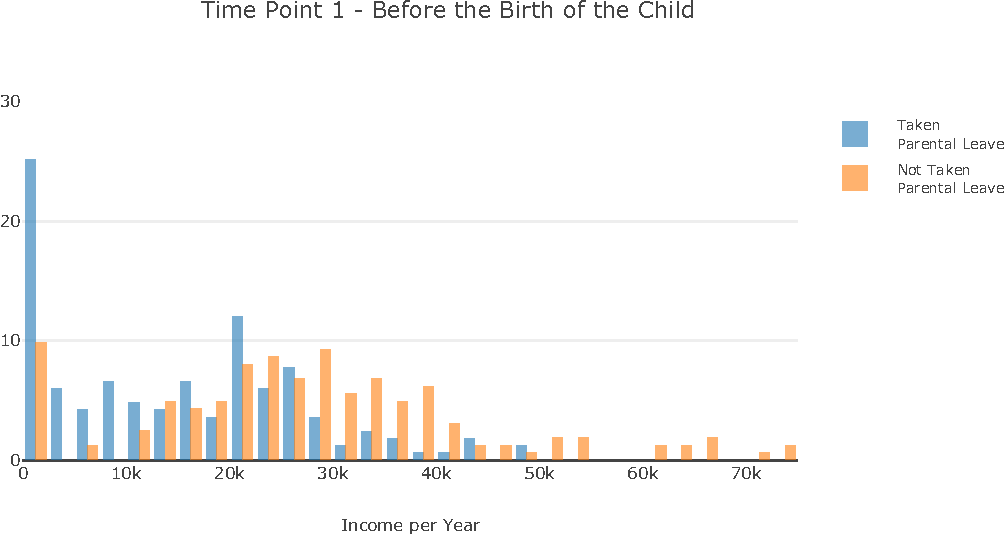
\includegraphics{Parental_Leave-Finalizing-Data-Set_files/figure-latex/fig-1-1} 

}

\caption{Distribution of Income}\label{fig:fig-1}
\end{figure}

\begin{figure}

{\centering 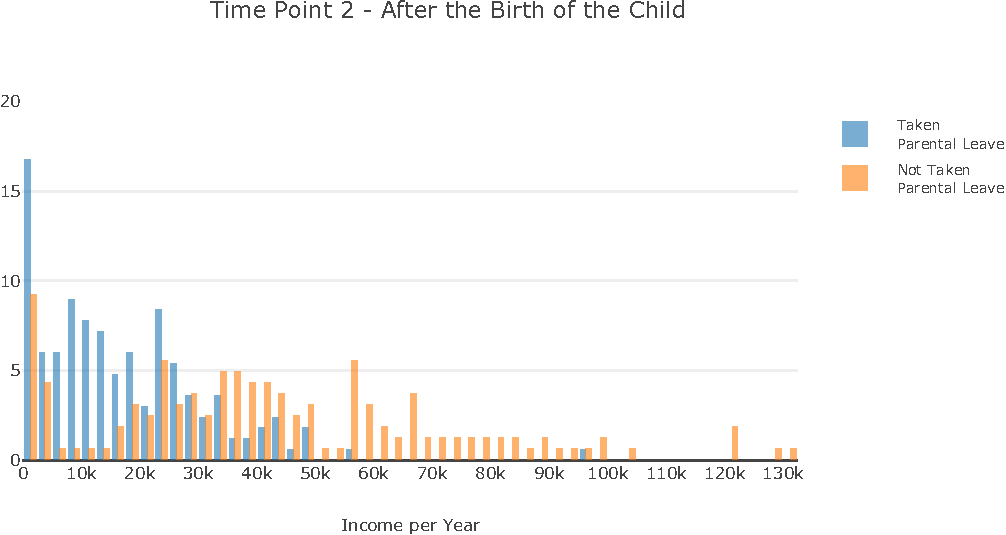
\includegraphics{Parental_Leave-Finalizing-Data-Set_files/figure-latex/fig-2-1} 

}

\caption{Distribution of Income}\label{fig:fig-2}
\end{figure}

\begin{table}[!htbp] \centering 
  \caption{Regression table for Hypothesis 1} 
  \label{tab2} 
\footnotesize 
\begin{tabular}{@{\extracolsep{-5pt}}lcccc} 
\\[-1.8ex]\hline 
\hline \\[-1.8ex] 
 & \multicolumn{4}{c}{\textit{Dependent variable:}} \\ 
\cline{2-5} 
\\[-1.8ex] & \multicolumn{4}{c}{Annual Income} \\ 
 & M1 & M2 & M3 & M4 \\ 
\hline \\[-1.8ex] 
 Parental Leave & $-$12,399.040$^{***}$ & $-$7,984.528$^{*}$ & $-$5,489.348 & $-$8,744.180$^{*}$ \\ 
  & (2,099.990) & (4,661.177) & (4,843.517) & (5,016.677) \\ 
  & & & & \\ 
 Male &  & 7,014.564 & 7,832.613 & 6,229.043 \\ 
  &  & (4,725.737) & (4,874.618) & (5,099.879) \\ 
  & & & & \\ 
 Age &  & 3,200.347 &  & 3,186.185 \\ 
  &  & (2,057.393) &  & (2,060.677) \\ 
  & & & & \\ 
 Age Squared &  & $-$57.642$^{*}$ &  & $-$57.503$^{*}$ \\ 
  &  & (30.259) &  & (30.305) \\ 
  & & & & \\ 
 West Germany &  & $-$963.382 &  & $-$1,026.475 \\ 
  &  & (2,637.065) &  & (2,645.316) \\ 
  & & & & \\ 
 Child Count &  & 1,014.902 &  & 1,029.209 \\ 
  &  & (1,251.661) &  & (1,253.963) \\ 
  & & & & \\ 
 High Education &  & 12,396.130$^{***}$ &  & 12,468.090$^{***}$ \\ 
  &  & (2,346.398) &  & (2,356.257) \\ 
  & & & & \\ 
 Occupation &  & $-$809.866$^{**}$ &  & $-$796.397$^{**}$ \\ 
  &  & (344.886) &  & (346.922) \\ 
  & & & & \\ 
 Parental Leave X Male &  &  & 599.617 & 5,732.633 \\ 
  &  &  & (14,378.260) & (13,867.910) \\ 
  & & & & \\ 
 Constant & 14,695.790$^{***}$ & $-$32,755.410 & 7,685.118$^{*}$ & $-$31,797.130 \\ 
  & (1,496.158) & (33,625.810) & (4,611.764) & (33,754.530) \\ 
  & & & & \\ 
\hline \\[-1.8ex] 
Observations & 329 & 294 & 329 & 294 \\ 
Adjusted R$^{2}$ & 0.094 & 0.200 & 0.096 & 0.198 \\ 
\hline 
\hline \\[-1.8ex] 
\textit{Note:}  & \multicolumn{4}{r}{$^{*}$p$<$0.1; $^{**}$p$<$0.05; $^{***}$p$<$0.01} \\ 
\end{tabular} 
\end{table}

\begin{figure}

{\centering 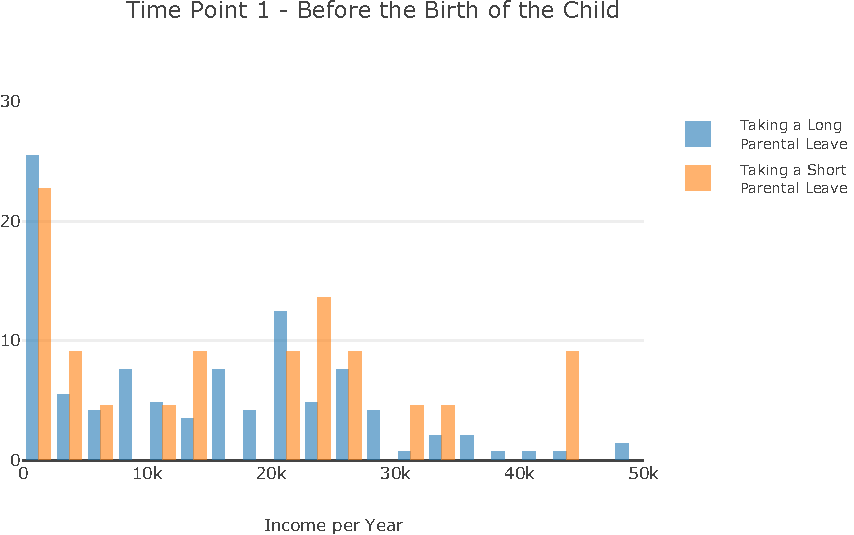
\includegraphics{Parental_Leave-Finalizing-Data-Set_files/figure-latex/fig-3-1} 

}

\caption{Distribution of Income}\label{fig:fig-3}
\end{figure}

\begin{figure}

{\centering 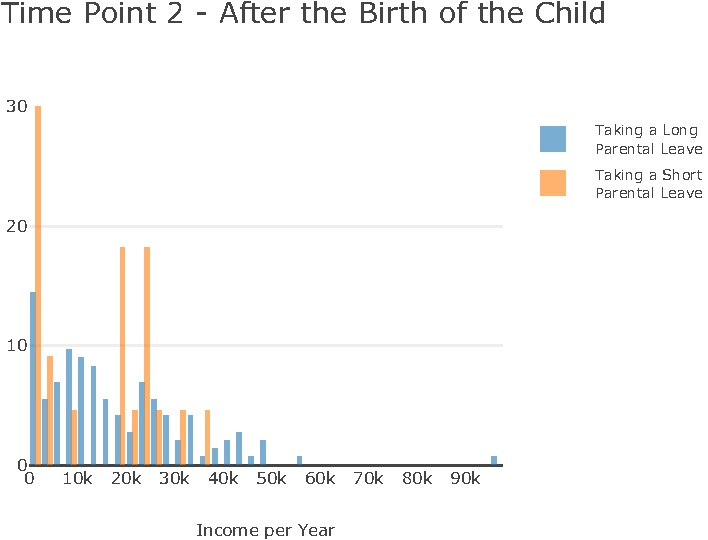
\includegraphics{Parental_Leave-Finalizing-Data-Set_files/figure-latex/fig-4-1} 

}

\caption{Distribution of Income}\label{fig:fig-4}
\end{figure}

\begin{table}[!htbp] \centering 
  \caption{Regression table for Hypothesis 1} 
  \label{tab2} 
\footnotesize 
\begin{tabular}{@{\extracolsep{-5pt}}lcc} 
\\[-1.8ex]\hline 
\hline \\[-1.8ex] 
 & \multicolumn{2}{c}{\textit{Dependent variable:}} \\ 
\cline{2-3} 
\\[-1.8ex] & \multicolumn{2}{c}{Annual Income} \\ 
 & M1 & M2 \\ 
\hline \\[-1.8ex] 
 Long Leave & 6,486.803$^{*}$ & 5,477.542 \\ 
  & (3,624.890) & (3,533.875) \\ 
  & & \\ 
 Male &  & 8,828.225 \\ 
  &  & (10,971.770) \\ 
  & & \\ 
 Age &  & 6,417.928$^{**}$ \\ 
  &  & (3,047.421) \\ 
  & & \\ 
 Age Squared &  & $-$99.910$^{**}$ \\ 
  &  & (48.740) \\ 
  & & \\ 
 West Germany &  & $-$9,023.413$^{***}$ \\ 
  &  & (2,907.949) \\ 
  & & \\ 
 Child Count & $-$3,335.500 & $-$96,482.760$^{**}$ \\ 
  & (3,377.696) & (47,191.880) \\ 
  & & \\ 
\hline \\[-1.8ex] 
Observations & 167 & 167 \\ 
Adjusted R$^{2}$ & 0.013 & 0.072 \\ 
\hline 
\hline \\[-1.8ex] 
\textit{Note:}  & \multicolumn{2}{r}{$^{*}$p$<$0.1; $^{**}$p$<$0.05; $^{***}$p$<$0.01} \\ 
\end{tabular} 
\end{table}

\hypertarget{refs}{}
\leavevmode\hypertarget{ref-becker_human_1993}{}%
Becker, Gary S. 1993. \emph{Human Capital: A Theoretical and Empirical Analysis, with Special Reference to Education}. 3rd ed. Chicago: The University of Chicago Press.

\leavevmode\hypertarget{ref-evertsson_parental_2016}{}%
Evertsson, Marie. 2016. ``Parental Leave and Careers: Women's and Men's Wages After Parental Leave in Sweden.'' \emph{Advances in Life Course Research} 29:26--40.

\leavevmode\hypertarget{ref-gabriele_mari_parental_2019}{}%
Gabriele Mari and Giorgio Cutuli. 2019. ``Do Parental Leaves Make the Motherhood Wage Penalty Worse? Assessing Two Decades of German Reforms.'' \emph{Deutsches Institut F\textbackslash"\{u\}r Wirtschaftsforschung (DIW)} 1025:http://hdl.handle.net/10419/194106.

\leavevmode\hypertarget{ref-geisler_against_2011}{}%
Geisler, Esther and Michaela Kreyenfeld. 2011. ``Against All Odds: Fathers' Use of Parental Leave in Germany.'' \emph{Journal of European Social Policy} 21(1):88--99.

\leavevmode\hypertarget{ref-helen_dearing_does_2015}{}%
Helen Dearing. 2015. ``Does Parental Leave Influence the Gender Dividon of Labour? Recent Empirical Findings from Europe.''

\leavevmode\hypertarget{ref-hofferth_parental_2006}{}%
Hofferth, Sandra L. and Sally C. Curtin. 2006. ``Parental Leave Statutes and Maternal Return to Work After Childbirth in the United States.'' \emph{Work and Occupations} 33(1):73--105.

\leavevmode\hypertarget{ref-katherine_marshall_fathers_2008}{}%
Katherine Marshall. 2008. ``Fathers' Use of Paid Parental Leave.'' \emph{Statistics Canada} 75-001-X.

\leavevmode\hypertarget{ref-lapuerta_individual_2011}{}%
Lapuerta, Irene, Pau Baizán, and María José González. 2011. ``Individual and Institutional Constraints: An Analysis of Parental Leave Use and Duration in Spain.'' \emph{Population Research and Policy Review} 30(2):185--210.

\leavevmode\hypertarget{ref-marshall_fathers_2008}{}%
Marshall, Katherine. 2008. ``Father's Use of Paid Parental Leave.'' \emph{Perspectives on Labour and Income} 9.

\leavevmode\hypertarget{ref-pronzato_return_2009}{}%
Pronzato, Chiara Daniela. 2009. ``Return to Work After Childbirth: Does Parental Leave Matter in Europe?'' \emph{Review of Economics of the Household} 7(4):341--60.

\leavevmode\hypertarget{ref-rostgaard_parental_2020}{}%
Rostgaard, Tine, Mogens Christoffersen, and Hanne Weise. 2020. ``Parental Leave in Denmark.''

\leavevmode\hypertarget{ref-sundstrom_gender_2002}{}%
Sundstrom, M. 2002. ``Gender Division of Childcare and the Sharing of Parental Leave Among New Parents in Sweden.'' \emph{European Sociological Review} 18(4):433--47.

\leavevmode\hypertarget{ref-tamm_fathers_2018}{}%
Tamm, Marcus. 2018. \emph{Fathers' Parental Leave-Taking, Childcare Involvement and Mothers' Labor Market Participation}. RWI.

\end{document}
